\chapter{Homotopía. El grupo fundamental}

\section{Equivalencia homotópica}

\defn{Camino o arco}{
    Sea ($X,\tau$) un espacio topológico e $I = [0,1] \subset \R$. Se llama \textbf{camino o arco} en $X$ a una aplicación continua $\alpha: I \to X$. Se llama $\alpha(0)$ origen y $\alpha(1)$ final. Diremos que $\alpha$ es un arco uniendo $\alpha(0)$ con $\alpha(1)$. Cuando $\alpha(0) = \alpha(1)$ diremos que $\alpha$ es un lazo.
}

\defn{Aplicaciones homotópicas}{
    Dos aplicaciones continuas $f ,g : X \to Y$ entre dos espacios topológicos son homotópicas si existe una aplicación continua $F : X \times [0,1] \to Y$ tal que $F(x,0) = f(x)$ y $F(x,1) = g(x)$, para todo $x \in X$. Se dice que $F$ es una homotopía entre $f$ y $g$, y se representa por $f \simeq g$.
}

\rmkb{
    Si $F$ es una homotopía, para cada $t \in [0,1]$, definimos $F_t : X \to Y$ por $F_t(x) = F(x,t)$. Las aplicaciones $F_t$ son continuas, $F_0 = f$ y $F_1 = g$. Si fijamos $x$, entonces
    \[
    F_x(t) = F(x,t) : I \to Y
    \]
    es un arco en $Y$ uniendo $f(x)$ con $g(x)$.
}

\clearpage

\ex{
    Si $Y\subset \R^n$ es convexo, cualquier par de aplicaciones $f,g$ continuas son homotópicas.
}

\pf{
    Consideremos la siguiente homotopía:
    \[
    F:X\times I \to Y,\quad F(x,t)=tg(x)+(1-t)f(x)
    \]
    como para cada $x\in X$ se tiene $f(x),g(x)\in Y$ y el conjunto $Y$ es convexo, entonces el segmento contenido entre $f(x),g(x)$ está contenido en $Y$, luego $F$ está bien definida. Además es continua por ser composición de aplicaciones continuas. Finalmente notemos que $F(x,0)=f(x),F(x,1)=g(x)$.
}

\ex{
    Sean $X, Y$ espacios topológicos e $y_1, y_2 \in Y$. Entonces las aplicaciones constantes
    \[
    C_{y_i} : X \to Y,\quad C_{y_i}(x) = y_i,\quad i=1,2
    \]
    son homotópicas si y solo si existe un arco en $Y$ uniendo $y_1, y_2$.
}

\pf{
    Si ambas aplicaciones son homotópicas sea $F(x,t)$ la homotopía entre ellas, entonces dado $x_0\in X$ arbitrario la aplicación $F_{x_0}(t)=F(x_0,t)$ es un camino que une $y_1,y_2$ puesto que es continua y
    \[
    F_{x_0}(0)=F(x_0,0)=C_{y_1}(x_0)=y_1,\quad F_{x_0}(1)=F(x_0,1)=C_{y_2}(x_0)=y_2.
    \]

    Si por el contrario existe $\alpha:I\to Y$ un camino uniendo $y_1=\alpha(0),y_2=\alpha(1)$ entonces consideremos la aplicación dada por
    \[
    F(x,t)=\alpha(t)
    \]
    que es claramente continua y además verifica $F(x,0)=y_1=C_{y_1}(x), F(x,1)=y_2=C_{y_2}(x)$, luego es una homotopía.
}

\propp{Relación $\simeq$ entre aplicaciones continuas}{
    La propiedad de ser homotópicas $\simeq$ es una relación de equivalencia en el conjunto $\mathcal{C}(X,Y)$ formado por todas las aplicaciones continuas de $X$ en $Y$. 
}{
    \textbf{1. Reflexiva:} $f \simeq f$

    Definamos la aplicación $F:X\times I\to Y$ por $F(x,t) = f(x)$. $F$ es continua por ser $f$ continua, además se tiene
    $\begin{cases}
        F(x,0) = f(x) \\
        F(x,1) = f(x)
    \end{cases}$
    por lo que es una homotopía, luego $f\simeq f$.

    \clearpage

    \noindent\textbf{2. Simétrica:} $f \simeq g \implies g \simeq f$
    
    Sea $F$ la homotopía entre $f,g$ entonces la aplicación
    \[
        \overline{F}:X\times I \to Y,\quad 
        \overline{F}(x,t) = F(x,1-t)
    \]
    es una homotopía entre $g,f$ puesto que es continua al serlo $F$ y cumple $\overline{F}(x,0)=F(x,1)=g(x), \overline{F}(x,1)=F(x,0)=f(x)$. 
    
    \textit{Nota:} La aplicación $\overline{F}$ se puede construir con cualquier homeomorfismo $\alpha : I \to I$ con $\alpha(0) = 1$ y $\alpha(1) = 0$ en vez de $1-t$.

    \noindent\textbf{3. Transitiva:} $f \simeq g,g \simeq h \implies f \simeq h$
    
    Sea $F_1$ la homotopía entre $f,g$ y $F_2$ la homotopía entre $g,h$, entonces la aplicación
    \[
    \overline{F}:X\times I \to Y,\quad
    \overline{F}(x,t) =\begin{cases}
        F_1(x,2t) & t \in [0, \frac{1}{2}] \\
        F_2(x,2t-1) & t \in [\frac{1}{2}, 1]
    \end{cases}
    \]
    es continua y verifica $\overline{F}(x,0)=F_1(x,0)=f(x), \overline{F}(x,1)=F_2(x,1)=h(x)$, por lo que es una homotopía entre $f$ y $h$.
    
    \textit{Nota:} Al igual que antes, se podría hacer con cualquier homeomorfismo que cumpla con lo que necesitamos.
}

\defn{Espacios homotópicamente equivalentes}{
    Decimos que dos espacios topológicos $X$ e $Y$ son homotópicamente equivalentes o tienen el mismo tipo de homotopía (denotado $X \simeq Y$) si existen aplicaciones continuas $f : X \to Y$ y $g :Y \to X$ tales que $g \circ f \simeq Id_X$ y $f \circ g \simeq Id_Y$. A la aplicación $f$ (también a $g$) se le llama, equivalencia de homotopía.
}

\ex{
    Si $Y \subset \R^n$ es convexo, entonces $Y \simeq \{x\}$.
}

\pf{
    Sea $X=\{x\}$, fijemos un $y_0\in Y$ y definamos las aplicaciones $f : X \to Y,\quad f(x)=y_0$ y $g : Y \to X,\quad g(y)=x$. Es inmediato notar que $g\circ f=Id_X$ puesto que para el único punto de $X$ se cumple
    \[
    g(f(x))=g(y_0)=x.
    \]
    Por tanto $g\circ f=Id_X\simeq Id_X$ por la reflexividad de $\simeq$.
    
    Por otro lado sea $h=f\circ g:Y\to Y$ y definamos la siguiente homotopía:
    \[
    H(y,t)= (y,t) = ty + (1-t)y_0 \implies
    \begin{cases}
        H(y,0) = y_0 = f(x) = f(g(y)) = h(y) \\
        H(y,1) = y = Id_Y(y)
    \end{cases}
    \]
    que es claramente continua y está bien definida porque $Y$ es convexo. 
}

\ex{
    $\R^2\setminus\{0\} \simeq \mathbb{S}^1$.
}

\pf{
    Buscamos $f : \R^2\setminus\{0\} \to \mathbb{S}^1$ y $g : \mathbb{S}^1 \to \R^2\setminus\{0\}$ continuas tales que
    \[
    \begin{cases}
        f \circ g \simeq Id_{\mathbb{S}^1} \\
        g \circ f \simeq Id_{\R^2\setminus\{0\}}.
    \end{cases}
    \]
    
    Sean $f(y) = \frac{y}{|y|}$ y $g(x) = x$. Es inmediato notar que $f\circ g= Id_{\mathbb{S}^1} \simeq Id_{\mathbb{S}^1}$ ya que \[
    f(g(x))=f(x)=\frac{x}{|x|}=x
    \]
    al ser $g(x)=x$ de norma 1.
    
    Por otro lado definamos la homotopía $F$ siguiente
    \[
        F(y,t)=ty + (1-t)\frac{y}{|y|},\quad
        \begin{cases}
            F(y,0) = \frac{y}{|y|}=g(f(y)) \\
            F(y,1) = y = Id_{\R^2\setminus\{0\}}(y)
        \end{cases}
    \]
    luego $g\circ f\simeq Id_{\R^2\setminus\{0\}}$.
}

\ex{
    La corona circular $C = \{(x,y) \in \R^2 : 1 \le x^2 +y^2 \le 2\} \simeq \mathbb{S}^1$
}
\pf{
    Procedemos de forma idéntica al ejemplo anterior. De hecho, se recomienda al lector intentar hacerlo como ejercicio antes de ver la solución.
    
    Definimos $f:C \to \mathbb{S}^1$, $g:\mathbb{S}^1 \to C$ como sigue:
    \begin{center}
        $f(y) = \frac{y}{|y|}$ \quad,\quad  $g(x) = x$
    \end{center}
    Para cualquier $x \in \mathbb{S}^1 $ se tiene que 
    \[
        f \circ g (x) = f(x) = x
    \] 
    Concluimos que $f \circ g = Id_{\mathbb{S}^1} \implies f \circ g \simeq Id_{\mathbb{S}^1}$. Por otro lado, si $y \in C$, 
    \[
    g\circ f (y) = g(\frac{y}{|y|}) = \frac{y}{|y|}
    \]
    Consideramos la homotopía $F : C \times I \to C$ siguiente, 
    \[
        F(y, t) = ty + (1 - t) \frac{y}{|y|}, \quad
        \begin{cases}
            F(y,0) = \frac{y}{|y|}=g(f(y)) \\
            F(y,1) = y = Id_{C}(y)
        \end{cases}
    \]
    Se puede comprobar fácilmente que para cualquier $y\in C$ la aplicación $F_y$ definida como $F_y(t) = F(y, t)$ verifica $F_y(t) \in C \quad \forall t \in I $. Así, $F$ está bien definida y por tanto $g\circ f \simeq Id_C$.
}


\propp{Espacios homeomorfos y homotopía}{
    Si $X$ e $Y$ son homeomorfos, entonces $X \simeq Y$. El recíproco no es cierto.
}{
    Supongamos que $X$ e $Y$ son homeomorfos. En tal caso existe $f:X \to Y$ homeomorfismo, que será una aplicación continua y con inversa $g=f^{-1}$ también continua. Entonces
    \[
    g\circ f=Id_{X}\simeq Id_X,\quad f\circ g=Id_{Y}\simeq Id_{Y}
    \]
    por lo que $X\simeq Y$.

    Como contraejemplo para el recíproco consideremos el conjunto $\R^n$ que es convexo, por tanto $\R^n\simeq \{x\}$ para cualquier $x\in\R^n$, sin embargo no son espacios homeomorfos puesto que $\R^n$ no es compacto y $\{x\}$ sí.
}

\propp{Relación $\simeq$ entre espacios}{
    La propiedad $\simeq$ define una relación de equivalencia entre los espacios topológicos.
}{
    \textbf{1. Reflexiva:} $X \simeq X$
    
    Basta tomar $f = g = Id_X \implies f \circ g = g \circ f = Id_X \simeq Id_X$.

    \noindent\textbf{2. Simetrica:} $X \simeq Y \implies Y \simeq X$
    
    Si $X \simeq Y$ entonces $\exists f:X\to Y, g:Y\to X$ de manera que $f \circ g \simeq Id_X, g \circ f \simeq Id_Y$, luego tomando $\bar{f}=g, \bar{g}=f$ tenemos dos aplicaciones que cumplen lo necesario para que $Y \simeq X$.

    \noindent\textbf{3. Transitiva:} $X \simeq Y, Y \simeq Z \implies X \simeq Z$
    
    Por hipótesis $\exists f_1:X\to Y, g_1:Y\to X$ cumpliendo
    \[
    f_1 \circ g_1 \simeq Id_X, g_1 \circ f_1 \simeq Id_Y
    \]
    y también $\exists f_2:Y\to Z, g_2:Z\to Y$ de manera que
    \[
    f_2 \circ g_2 \simeq Id_Y, g_2 \circ f_2 \simeq Id_Z
    \]
    Definamos ahora
    \[
    f=f_2\circ f_1: X \to Z,\quad g=g_1\circ g_2: Z \to X
    \]
    y notemos que se tiene:\footnote{Para los pasos $\simeq$ ver el Ejercicio 3.1}
    \[
    f\circ g = f_2\circ f_1\circ g_1\circ g_2 \simeq f_2\circ Id_Y \circ g_2 = f_2\circ g_2 \simeq Id_Z
    \]
    así como
    \[
    g\circ f =g_1\circ g_2\circ f_2\circ f_1 \simeq g_1\circ Id_Y\circ f_1 = g_1\circ f_1 \simeq Id_X.
    \]

    \textit{Nota: A lo largo de la demostración todas las aplicaciones que aparecen son continuas, recordemos que esto es indispensable para que podamos hablar de homotopías.}
}

\exer{
    Probar que si $f_1: X \to Y, f_2: X \to Y, g: Y \to Z$ son aplicaciones continuas tales que $f_1 \simeq f_2$ entonces se tiene $g \circ f_1 \simeq g \circ f_2$. Plantear y resolver el problema análogo para ver que se cumple $f_1 \circ g \simeq f_2 \circ g$
}

\clearpage

\section{Espacios contractiles}

\defn{Espacio contráctil}{
    Un espacio topológico X se dice que es contráctil si es homotópicamente equivalente a un punto.
}

\propp{Caracterizaciones de espacios contráctiles}{
    Sea $Y$ un espacio topológico, las siguientes afirmaciones son equivalentes:
    \begin{enumerate}
        \item $Y$ es contráctil.
        \item Existe $y_0 \in Y$ tal que $Id_Y$ y $C_{y_0}:Y\to \{y_0\}$ son homotópicas.
        \item Si $X$ es otro espacio topológico, cualquier par de aplicaciones continuas $f,g : X \to Y$ son homotópicas.
        \item Para todo $y_0\in Y$, se tiene que $C_{y_0}$ es homotópica a la $Id_Y$.
        \item Si $X$ es otro espacio topológico y $f:Y\to X$ continua, entonces existe $x_0\in X$ tal que $f \simeq C_{x_0}$. 
    \end{enumerate}
}{
    (1$\implies$2)
    
    Por hipótesis $Y \simeq \{p\}$, luego existen aplicaciones $g:Y\to \{p\}, f:\{p\}\to Y$ cumpliendo que $g\circ f \simeq Id_{\{p\}}$ y $f\circ g \simeq Id_Y$. Notemos que $g$ debe ser $C_p$, es decir $g(y)=p$ $\forall y\in Y$ ya que el espacio de llegado es un único punto, y por otro lado la imagen de $f$ será un único punto $f(p)=y_0$.
    
    Notemos ahora que dado $y \in Y$, $f(g(y))=f(p)=:y_0\in Y$, luego $C_{y_0} = f \circ g \simeq Id_Y$, por tanto existe $y_0=f(p)$ de manera que $Id_Y \simeq C_{y_0}$.

    \noindent(2$\implies$3)
    
    Sabemos que $\exists y_0\in Y$ tal que $Id_Y \simeq C_{y_0}$. Sea $X$ espacio topológico, y $f,g:X\to Y$ continuas. Veamos que $f \simeq g$.
    $$ f = Id_Y\circ f \simeq C_{y_0}\circ f = \overline{C_{y_0}} :X \to \{y_0\} \text{ tal que } \overline{C_{y_0}}(x) = y_0 $$
    $$ g = Id_Y\circ g \simeq C_{y_0}\circ g = \overline{C_{y_0}} :X \to \{y_0\} \text{ tal que } \overline{C_{y_0}}(x) = y_0 $$

    Por tanto, $f \simeq \overline{C_{y_0}} \simeq g$.

    \noindent (3$\implies$4)
    
    Tomemos $Y=X,\ f=Id_Y,\ g=C_{y_0}$, con $y_0\in Y$ arbitrario. Aplicando (3) a estos espacios y funciones se obtiene que $Id_Y = f \simeq g = C_{y_0}$.

    \noindent (4$\implies$5)
    
    Sabemos que $C_{y_0} \simeq Id_Y, \forall y_0\in Y$. Sea $X$ espacio topológico y $f:Y\to X$ continua. Entonces
    \[
    f = f\circ Id_Y \simeq f\circ C_{y_0} : Y \to X
    \]
    donde $(f\circ C_{y_0})(y) = f(C_{y_0}(y)) = f(y_0)$. Luego, $f\circ C_{y_0} = C_{f(y_0)}:Y\to X$. Tomando $x_0 = f(y_0)$, se tiene que $f \simeq C_{x_0}$. 

    \noindent (5$\implies$2)
    
    Aplicamos la hipótesis al espacio $X=Y$ y la función $f=Id_Y$. Entonces, obtenemos $y_0\in Y$ tal que $f\simeq C_{y_0}$. Por tanto, $Id_Y \simeq C_{y_0}$.

    \noindent (2$\implies$1)
    
    Por la hipótesis, existe $y_0\in Y$ tal que $Id_Y \simeq C_{y_0}$. Las aplicaciones buscadas son
    \begin{align*}
        &f = C_{y_0} : Y \to \{y_0\},\quad f(y)=y_0 \\
        &g = \iota : \{y_0\} \to Y,\quad g(y_0)=y_0
    \end{align*}
    que son continuas y cumplen:
    \begin{align*}
        f \circ g &= Id_{\{y_0\}} \simeq Id_{\{y_0\}} \\
        g \circ f &= C_{y_0} \simeq Id_{Y}
    \end{align*}
    luego $Y\simeq \{y_0\}$.
}

\corp{
    Todo espacio contráctil es arcoconexo y por tanto conexo.
}{\label{cor:contractil-arcoconexo}
    Sea $Y$ un espacio contráctil y sean $y_1,y_2 \in Y$ dos puntos arbitrarios. Aplicando el apartado (3) de la proposición anterior a las aplicaciones $f=C_{y_1},g=C_{y_2}:Y\to Y$ continuas obtenemos
    \[
    C_{y_1} \simeq C_{y_2} \iff \exists F:Y\times I \to Y \text{ continua tal que } \begin{cases}
        F(y,0) = C_{y_1}(y) = y_1 \\
        F(y,1) = C_{y_2}(y) = y_2
    \end{cases}
    \]
    Consideremos la aplicación $\alpha:I \to Y, \alpha(t) = F(y_0,t)$, con $y_0\in Y$ fijo. Esta aplicación es claramente continua y une $y_1$ y $y_2$, por tanto, $Y$ es arcoconexo.
}

\defn{Invariante homotópico}{
    Un invariante homotópico es una propiedad topológica $\partes$ que se conserva por equivalencias homotópicas, es decir, si $X \simeq Y$, entonces $X$ satisface $\partes$ si, y solo si, $Y$ satisface $\partes$.
}

\ex{
    \begin{enumerate}
        \item La conexión es un invariante homotópico.
        \item La conexión por caminos es un invariante homotópico.
        \item La compacidad NO es un invariante homotópico.
    \end{enumerate}
}

\clearpage

\section{Homotopía por caminos}

\defn{Caminos homotópicos}{
    Dos caminos $\alpha,\beta : I \to X$ en un espacio topológico $X$ uniendo dos puntos $x_0$ y $x_1$ se dice que son homotópicos (por caminos) si existe una homotopía $F : I \times I \to X$ entre $\alpha$ y $\beta$ tal que $F(0,t) = x_0$, $F(1,t) = x_1$, para todo $t \in I$. Lo denotaremos por $\alpha \simeq_p \beta$.
}

\rmkb{
    El subíndice $p$ de $\simeq_p$ proviene de que en inglés camino se traduce por \textit{path}.
}

\rmkb{
    Para cada $t\in I$, $F_t$ es un camino uniendo $x_0$ y $x_1$, con $F_0 = \alpha$ y $F_1 = \beta$. En la siguiente imagen aparecen los distintos $F_t$ en color gris:
    \begin{center}
        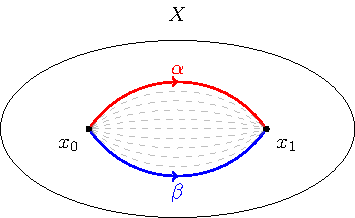
\includegraphics[]{img/homotopia-caminos}
    \end{center}
}

\rmkb{
    ¡Ojo! $F$ ahora está definida en $I\times I$, por lo que podría haber confusión al hablar de $F_t$ para $t\in I$ sin mencionar explícitamente qué componente de $F$ estamos fijando. Para nosotros, $t$ siempre será la variable de la segunda componente de $F$, y $s$ de la primera. Escribiremos $F_t(s) = F(s,t)$.
}

\propp{Relación de equivalencia $\simeq_p$}{
    $\simeq_p$ define una relación de equivalencia sobre el conjunto de caminos que unen $x_0,x_1$. Denotamos por $[\alpha]$ la clase asociada a un camino $\alpha$.
}{
    \textbf{1. Reflexiva:} $\alpha \simeq \alpha$

    Definamos la aplicación $F:I\times I \to X$ por $F(s,t) = \alpha(s)$. $F$ es continua por ser $\alpha$ continua, además se tiene
    $\begin{cases}
        F(s,0) = \alpha(s) \\
        F(s,1) = \alpha(s)
    \end{cases}$
    por lo que es una homotopía. Como además cumple
    \[
        F(0,t)=\alpha(0)=x_0, F(1,t)=\alpha(1)=x_1
    \]
    se tiene $\alpha \simeq_p \alpha$.

    \noindent\textbf{2. Simétrica:} $\alpha \simeq \beta \implies \beta \simeq \alpha$
    
    Sea $F$ la homotopía por caminos entre $\alpha, \beta$ entonces la aplicación
    \[
        \overline{F}: I \times I \to X,\quad 
        \overline{F}(s,t) = F(s,1-t)
    \]
    es una homotopía por caminos entre $\beta,\alpha$ puesto que es continua al serlo $F$ y cumple
    \[
    \overline{F}(s,0)=F(s,1)=\beta(s), \overline{F}(s,1)=F(s,0)=\alpha(s)
    \]
    así como
    \[
    \overline{F}(0,t) = F(0,1-t) = x_0, \overline{F}(1,t) = F(1,1-t) = x_1
    \]
    por tanto $\beta \simeq_p \alpha$.

    \noindent\textbf{3. Transitiva:} $\alpha \simeq \beta,\beta \simeq \gamma \implies \alpha \simeq \gamma$
    
    Sea $F_1$ la homotopía por caminos entre $\alpha,\beta$ y $F_2$ la homotopía por caminos entre $\beta,\gamma$, entonces la aplicación
    \[
    \overline{F}:I \times I \to X,\quad
    \overline{F}(s,t) =\begin{cases}
        F_1(s,2t) & t \in [0, \frac{1}{2}] \\
        F_2(s,2t-1) & t \in [\frac{1}{2}, 1]
    \end{cases}
    \]
    es continua y verifica $\overline{F}(s,0)=F_1(s,0)=\alpha(s), \overline{F}(s,1)=F_2(s,1)=\gamma(s)$, y también
    \[
        \overline{F}(0,t) = \begin{cases}
            F_1(0,2t)=x_0 & t \in [0, \frac{1}{2}] \\
            F_2(0,2t-1)=x_0 & t \in [\frac{1}{2}, 1]
        \end{cases},\quad
        \overline{F}(1,t) = \begin{cases}
            F_1(1,2t)=x_1 & t \in [0, \frac{1}{2}] \\
            F_2(1,2t-1)=x_1 & t \in [\frac{1}{2}, 1]
        \end{cases}
    \]
    por lo que es una homotopía entre $\alpha$ y $\gamma$.
}

\defn{Producto de caminos}{
    Si $\alpha$ es un camino uniendo $x_0$ y $x_1$, y $\beta$ es un camino uniendo $x_1$ y $x_2$, definimos el camino producto $\alpha * \beta$ por 
    \[
        \alpha * \beta(s) =
        \begin{cases}
            \alpha(2s) & s \in [0, \frac{1}{2}] \\
            \beta(2s - 1) & s \in [\frac{1}{2}, 1]
        \end{cases}
    \]
}

\rmkb{
    Es importante tener en mente que definimos el producto de caminos de izquierda a derecha, es decir, recorriendo primero el camino de la izquierda y después el de la derecha.
}


\lemp{Lema previo}{
    Sea $\alpha$ un camino uniendo $x_0$ y $x_1$, sea $\beta$ un camino uniendo $x_1$ y $x_2$. Entonces, para cualquier $r\in(0,1)$ se cumple $\alpha*\beta \simeq_p \gamma,\quad \gamma(t) = \begin{cases}
        \alpha(\frac{t}{r}) & t \in [0, r] \\
        \beta(\frac{t-r}{1-r}) & t \in [r, 1].
    \end{cases}$
}{
    Queremos ver que $\alpha*\beta$ y $\gamma$ son homotópicos por caminos, luego necesitamos una homotopía $H:I\times I \to X$ tal que $H(x,0) = \alpha*\beta(x)$ y $H(x,1) = \gamma(x)$, y además $H(0,t) = x_0$ y $H(1,t) = x_2$.
    
    Definamos $H$ de la siguente manera
    \[
    H(x,t) = \begin{cases}
        \alpha\Big(\frac{x}{(1-t)\frac{1}{2}+tr}\Big) & x \in [0, (1-t)\frac{1}{2}+tr] \\
        \beta\Big(\frac{x-(1-t)\frac{1}{2}-tr}{1-(1-t)\frac{1}{2}-tr}\Big) & x \in [(1-t)\frac{1}{2}+tr, 1]
    \end{cases}
    \]
    Claramente $H$ es continua por el lema del pegado y además se verifican las siguientes propiedades que necesitabamos comprobar:
    \begin{itemize}
        \item $H(x,0) = \alpha*\beta(x) \checkmark$
        \item $H(x,1) = \gamma(x) \checkmark$
        \item $H(0,t) = \alpha(0) = x_0 \checkmark$
        \item $H(1,t) = \beta(1) = x_2 \checkmark$
    \end{itemize}
}

\propp{Propiedades del producto de caminos}{
    \label{prop:propiedades-producto-caminos}
    \begin{enumerate}
        \item $\alpha * (\beta * \gamma) \simeq_p (\alpha * \beta) * \gamma$.
        \item Si $\epsilon_{x_0}$ es el arco constante $x_0$ y $\epsilon_{x_1}$ el arco constante $x_1$, entonces
        \[
            \epsilon_{x_0} * \alpha \simeq_p \alpha \text{ y } \alpha * \epsilon_{x_1} \simeq_p \alpha
        \]
        \item Sea $\bar{\alpha}(t) = \alpha(1-t), t\in I$. Entonces, $$\alpha * \bar{\alpha} \simeq_p \epsilon_{x_0} \text{ y } \bar{\alpha} * \alpha \simeq_p \epsilon_{x_1}$$
    \end{enumerate}
}{
    \begin{enumerate}
        \item Es inmediato notar que
        \begin{align*}
            \alpha * (\beta * \gamma)(s) &=
            \begin{cases}
                \alpha(2s) & s \in [0, \frac{1}{2}] \\
                \beta(4s-2) & s \in [\frac{1}{2}, \frac{3}{4}]\\
                \gamma(4s-3) & s \in [\frac{3}{4}, 1]
            \end{cases}\\
            (\alpha * \beta) * \gamma(s) &=
            \begin{cases}
                \alpha(4s) & s \in [0, \frac{1}{4}] \\
                \beta(4s-1) & s \in [\frac{1}{4}, \frac{1}{2}]\\
                \gamma(2s-1) & s \in [\frac{1}{2}, 1]
            \end{cases}
        \end{align*}
        Aplicando el lema previo con $r=\frac{1}{3}$ al primer producto obtenemos
        \[
            \alpha * (\beta * \gamma)(s) \simeq_p \sigma(s)=
            \begin{cases}
                \alpha(3s) & s \in [0, \frac{1}{3}] \\
                \beta(3s-1) & s \in [\frac{1}{3}, \frac{2}{3}]\\
                \gamma(3s-2) & s \in [\frac{2}{3}, 1]
            \end{cases}
        \]
        y de nuevo aplicandolo al segundo producto se puede llegar a $(\alpha * \beta) * \gamma(s) \simeq_p \sigma(s)$, lo que prueba finalmente que $\alpha * (\beta * \gamma) \simeq_p \sigma \simeq_p (\alpha * \beta) * \gamma$.

        \item Probaremos solo el primer caso, el segundo es muy similar. Definamos la siguiente aplicación 
        \[
        H(x,t) = \begin{cases}
            x_0 & x \in [0, \frac{t}{2}] \\
            \alpha\Big(\frac{2x-t}{2-t}\Big) & x \in [\frac{t}{2}, 1]
        \end{cases}
        \]
        que es una homotopía por caminos puesto que es continua y verifica
        \[
        H(x,1)=\epsilon_{x_0} * \alpha(x), H(x,0)=\alpha(x), H(0,t)=x_0, H(1,t)=x_1,
        \]
        luego $\alpha\simeq_p\epsilon_{x_0} * \alpha$.

        \item De nuevo probamos solo el primer caso, para ello basta definir la siguiente homotopia por caminos $H:I\times I\to X$, dada por
        \[
            H(x, t) = 
            \begin{cases} 
            \alpha(2x(1-t)) & x \in [0, \frac{1}{2}] \\
            \alpha((2-2x)(1-t)) & x \in [\frac{1}{2}, 1]
            \end{cases}
        \]
        esta aplicación es continua y efectivamente cumple $H(x,1)=\epsilon_{x_0}(x), H(0,t)=x_0, H(1,t)=x_0$, además de
        \[
        H(x,0)=
        \begin{cases} 
            \alpha(2x) & x \in [0, \frac{1}{2}] \\
            \alpha(2-2x)=\alpha(1-(2x-1))=\bar{\alpha}(2x-1) & x \in [\frac{1}{2}, 1]
            \end{cases}
        =\alpha * \bar{\alpha}(x).
        \]
    \end{enumerate}
}

\defn{Conjunto de arcos}{
    Dado $X$ un espacio topológico, denotaremos por $$\Omega_{x_0}^{x_1}(X) := \{\alpha:I\to X \text{ continua con } \alpha(0) = x_0, \alpha(1)=x_1\}$$ y $$\Omega_{x_0} = \Omega_{x_0}^{x_0}(X)$$
    Llamaremos $$\pi_1(X,x_0) : \faktor{\Omega_{x_0}}{\simeq_p}$$
}

\propp{Producto de clases de homotopía}{
    El producto $*$ induce un producto bien definido para clases de homotopía:
    $$[\alpha]*[\beta]:=[\alpha*\beta]$$
}{
    Veamos que el producto $*$ está bien definido en el cociente, es decir, no depende de los representantes elegidos de las clases $[\alpha]$ y $[\beta]$. Sean $\alpha_1, \alpha_2 \in \Omega_{x_0}^{x_1}$ con $\alpha_1 \simeq_p \alpha_2$ y $\beta_1, \beta_2 \in \Omega_{x_1}^{x_2}$ con $\beta_1 \simeq_p \beta_2$. Queremos probar que $\alpha_1 * \beta_1 \simeq_p \alpha_2 * \beta_2$. Llamemos $F_{\alpha}$ a la homotopía entre $\alpha_1$ y $\alpha_2$, y sea $F_{\beta}$ la homotopía entre $\beta_1$ y $ \beta_2$. 

    Buscamos probar que $\alpha_1 * \beta_1 $ y $\alpha_2 * \beta_2$ son caminos homotópicos. Nuestra homotopía candidata es $G : I \times I \to X$ como
    \[
        G(s, t) =
        \begin{cases}
            F_{\alpha}(2s, t) & \text{si } s \in [0, \frac{1}{2}], \\
            F_{\beta}(2s - 1, t) & \text{si } s \in [\frac{1}{2}, 1].
        \end{cases}
    \]

    Veamos que $G$ es homotopía. Es claramente continua por serlo $F_{\alpha} $ y $F_{\beta}$ y coindicir cuando $s=\frac{1}{2}$, y además verifica
    \[ 
        G(s, 0) =
        \begin{cases}
            G(s, 0) = F_{\alpha}(2s, 0) = \alpha_1(2s) = \alpha_1 * \beta_1(s) \quad & \text{si } s \in [0,\frac{1}{2}] \\
            G(s, 0) = F_{\beta}(2s - 1, 0) = \beta_1(2s) = \alpha_1 * \beta_1(s) \quad & \text{si } s \in [\frac{1}{2}, 1] 
        \end{cases}
    \]
    \[
        G(s, 1) =
        \begin{cases}
            G(s, 1) = F_{\alpha}(2s, 1) = \alpha_2(2s) = \alpha_2 * \beta_2(s) \quad & \text{si } s \in [0,\frac{1}{2}] \\
            G(s, 1) = F_{\beta}(2s - 1, 1) = \beta_2(2s) = \alpha_2 * \beta_2(s) \quad & \text{si } s \in [\frac{1}{2}, 1] 
        \end{cases}
    \] 

    Por otro lado, también se verifica la condición de homotopía de caminos, pues $\alpha_1 \simeq_p \alpha_2$ implica que $G(0, t) = F_{\alpha}(0, t) = x_0$. Análogamente, se tiene que $G(1, t) = F_{\beta}(1, t) = x_2$.

    Concluimos entonces que $\alpha_1 * \beta_1  \simeq_p \alpha_2 * \beta_2$, y por tanto $[\alpha] * [\beta]$ no depende de los representantes de las clases $[\alpha]$ y $[\beta]$.
}

Veremos a continuación que la estructura $(\pi_1(X, x_0), *)$ forma lo que en álgebra se conoce como un grupo. Un grupo es, esencialmente, un conjunto con una operación que satisface ciertas reglas (asociatividad, existencia de un elemento neutro y de inversos para cada elemento). Para una introducción más formal a los conceptos que usaremos de teoría de grupos, se puede consultar el \hyperref[apendice:teoria-de-grupos]{Apéndice A}.

\thm{El grupo fundamental}{
    El conjunto $\pi_1(X,x_0)$ junto con la operación producto $*$ es un grupo, denominado el grupo fundamental de $X$ en $x_0$.
}
\pf{
    Veamos que la operación $*$ definida en el cociente $\Omega_{x_0} / \simeq_p$ es asociativa, tiene un elemento neutro y todo elemento tiene un inverso respecto a ella. En esencia, aplicaremos la proposición \hyperref[prop:propiedades-producto-caminos]{3.3.5} a la operación en el cociente, usando que está bien definida. 
    
    \textbf{Asociatividad. } Sean $[\alpha], [\beta], [\gamma] \in \pi_1(X, x_0)$. Queremos ver que $([\alpha] * [\beta]) * [\gamma] = [\alpha] * ([\beta] * [\gamma])$. Por definición de la operación en el cociente, esto es equivalente a probar que $[(\alpha * \beta) * \gamma] = [\alpha * (\beta * \gamma)]$. La proposición \hyperref[prop:propiedades-producto-caminos]{3.3.5} (1) nos dice que $(\alpha * \beta) * \gamma \simeq_p \alpha * (\beta * \gamma)$, lo que implica que sus clases de homotopía son iguales.

    \textbf{Elemento neutro. } Sea $\epsilon_{x_0}$ el camino constante en $x_0$. La proposición \hyperref[prop:propiedades-producto-caminos]{3.3.5} (2) establece que $\epsilon_{x_0} * \alpha \simeq_p \alpha$ y $\alpha * \epsilon_{x_0} \simeq_p \alpha$ (notemos que en este caso $x_1=x_0$). En términos de clases de homotopía, esto significa que $[\epsilon_{x_0}] * [\alpha] = [\alpha]$ y $[\alpha] * [\epsilon_{x_0}] = [\alpha]$. Por lo tanto, $[\epsilon_{x_0}]$ es el elemento neutro del grupo.

    \textbf{Elemento inverso. } Para cualquier $[\alpha] \in \pi_1(X, x_0)$, consideremos el camino inverso $\bar{\alpha}(t) = \alpha(1-t)$. La proposición \hyperref[prop:propiedades-producto-caminos]{3.3.5} (3) nos dice que $\alpha * \bar{\alpha} \simeq_p \epsilon_{x_0}$ y $\bar{\alpha} * \alpha \simeq_p \epsilon_{x_0}$. Esto se traduce en $[\alpha] * [\bar{\alpha}] = [\epsilon_{x_0}]$ y $[\bar{\alpha}] * [\alpha] = [\epsilon_{x_0}]$. Por lo tanto, $[\bar{\alpha}]$ es el inverso de $[\alpha]$.

    Como la operación $*$ es asociativa, tiene elemento neutro y todo elemento tiene inverso, $(\pi_1(X, x_0), *)$ es un grupo.
}

\ex{
    Si $X\subset \R^n$ convexo, entonces $\pi_1(X,x_0) = (0,+)$ (el grupo trivial) para todo $x_0\in X$. En particular $\pi_1(\R^n,x_0) = (0,+)$ y $\pi_1(B^n, x_0) = (0,+)$, donde $B^n$ es la bola unidad.
}

\pf{
    Veamos que dado $X\subset\R^n$ convexo y $x\in X$ cualquier camino $\alpha\in\Omega_{x}$ es homotópico por caminos al camino constante $\epsilon_x$, y por tanto el grupo fundamental debe ser el grupo trivial al tener $\faktor{\Omega_{x}}{\simeq_p}$ un único elemento. Para ver que $\alpha\simeq_p\epsilon_x$ basta considerar la homotopía por caminos
    \[
    H(s,t)=t\alpha(s)+(1-t)\epsilon_x(s)=t\alpha(s)+(1-t)x
    \]
    que en efecto es continua y verifica $H(s,0)=\epsilon_x(s),H(s,1)=\alpha(s),H(0,t)=x=H(1,t)$.
}

\ex{
    $\pi_1(\R,x) = (0,+)$.
}

\rmkb{
    En los ejemplos anteriores se abusa ligeramente del lenguaje y se indica que los grupos fundamentales <<son>> el grupo trivial ya que son isomorfos a él. De hecho, cualquier grupo con un solo elemento es isomorfo al grupo trivial. Por otro lado, se suele abusar de la notación representando al grupo trivial simplemente como 0 en lugar de $(0,+)$. 
}

\defn{}{
    Sea $\sigma$ un camino uniendo dos puntos $x_0, x_1 \in X$. Definimos
    \[
    \hat{\sigma} : \pi_1(X, x_0) \to \pi_1(X, x_1)
    \]
    por
    \[
    \hat{\sigma}([\gamma]) = [\overline{\sigma}] * [\gamma] * [\sigma].
    \]
}

\propp{Proposición 6.8}{\label{prop:iso-grupos}
    La aplicación $\hat{\sigma}$ es un isomorfismo de grupos para todo camino $\sigma$. 
}{
    En primer lugar es claro que para todo $[\gamma]\in\pi_1(X,x_0)$ la imagen $\hat{\sigma}([\gamma])=[\overline{\sigma}] * [\gamma] * [\sigma] = [\overline{\sigma} * \gamma * \sigma]$ pertenece a $\pi_1(X,x_1)$, ya que
    \[
        \overline{\sigma} * \gamma * \sigma
    \]
    es un camino que parte de $x_1$ y llega a $x_1$ (recordamos que se recorre primero $\overline{\sigma}$).

    Para ver que $\hat{\sigma}$ es biyectiva comprobaremos que tiene inversa dada por
    \[
    (\hat{\sigma})^{-1}=\widehat{(\overline{\sigma})}
    \]
    en efecto se tiene
    \begin{align*}
        \widehat{(\overline{\sigma})}(\hat{\sigma}([\gamma]))=[\sigma] * \hat{\sigma}([\gamma]) * [\overline{\sigma}]=[\sigma] * [\overline{\sigma}] * [\gamma] * [\sigma] * [\overline{\sigma}] = [\gamma]
    \end{align*}
    donde hemos usado las propiedades de grupo de $\pi_1(X,x_0)$. Para comprobar que $\widehat{(\overline{\sigma})}$ también es inversa por la derecha de $\hat{\sigma}$ seguimos un razonamiento similar que omitimos.

    Para ver que es un homomorfismo basta notar que
    \begin{align*}
        \hat{\sigma}([\gamma]) * \hat{\sigma}([\alpha]) = [\overline{\sigma}] * [\gamma] * [\sigma] * [\overline{\sigma}] * [\alpha] * [\sigma] = [\overline{\sigma}] * [\gamma] * [\alpha] * [\sigma] = \hat{\sigma}([\gamma] * [\alpha])
    \end{align*}
    usando de nuevo que $\pi_1(X,x_0)$ es un grupo.
}

\rmkb{
    Podemos pensar en $\hat{\sigma}$ como un isomorfismo que cambia el <<punto base>> del grupo fundamental.
}

\corp{
    Si $X$ es conexo por caminos, todos los grupos $\pi_1(X, x_0)$ son isomorfos entre sí. En este caso, podemos considerar el grupo fundamental $\pi_1(X)$, independiente del punto base.
}{
    Sea $x_0,x_1\in X$ dos puntos arbitrarios. Entonces, existe un camino $\sigma$ que une $x_0$ y $x_1$. Por la proposición anterior se tiene que $\hat{\sigma}$ (definida segun la definición 3.3.9) es un isomorfismo de grupos, luego $\pi_1(X,x_0) \cong \pi_1(X,x_1)$.
}

\section{Espacios simplemente conexos}

\defn{Espacio simplemente conexo}{
    Decimos que un espacio topológico $X$ es simplemente conexo si es conexo por caminos y $\pi_1(X) = 0$.
}

\ex{
    Si $X \subset \mathbb{R}^n$ es convexo, entonces $X$ es simplemente conexo.
}

\clearpage

\section{El homomorfismo inducido}

\defn{Homomorfismo inducido}{
    Sea $f : X \to Y$ una aplicación continua. Para todo punto $x_0 \in X$, $f$ induce una aplicación
    \[
    f_* : \pi_1(X, x_0) \to \pi_1(Y, f(x_0))
    \]
    definida por $f_*([\alpha]) = [f \circ \alpha]$, denominada el homomorfismo inducido.
}

\clmp{}{
    $f_*$ es un homomorfismo de grupos.
}{
    En primer lugar notemos que $f\circ\alpha$ es un lazo centrado en $f(x_0)$ por ser $f$ continua. Ahora basta notar que dados $[\alpha],[\beta]\in\pi_1(X)$ tenemos
    \[
        f_*([\alpha]) * f_*([\beta]) = [f \circ \alpha] * [f \circ \beta] = [(f \circ \alpha) * (f \circ \beta)] = [f \circ (\alpha * \beta)] = f_*([\alpha * \beta]).
    \]
    Los detalles de cada paso, especialmente de
    \[
        f \circ (\alpha * \beta) = (f \circ \alpha) * (f \circ \beta)
    \]
    quedan para el lector.
}

\propp{Propiedades del homomorfismo inducido}{
    \begin{enumerate}
        \item Si $f: X \to Y$ y $g: Y \to Z$ son continuas, entonces $(g \circ f)_* = g_* \circ f_*$.
        \item Para la identidad $Id_X: X \to X$ se tiene $(Id_X)_* = Id_{\pi_1(X,x_0)}.$
        \item Si $f$ es un homeomorfismo, entonces $f_*$ es un isomorfismo de grupos. Así, el grupo fundamental es un invariante topológico.
    \end{enumerate}
}{
    \begin{enumerate}
        \item Sea $[\alpha]\in\pi_1(X)$, entonces
        \[
            (g \circ f)_*([\alpha])=[(g\circ f)\circ \alpha] = [g\circ(f\circ\alpha)] = g_*([f\circ\alpha]) = g_*(f_*([\alpha])) = g_* \circ f_* ([\alpha]).
        \]
        \item Es inmediato verificar que
        \[
            (Id_X)_*([\alpha]) = [Id_X \circ \alpha] = [\alpha] = Id_{\pi_1(X,x_0)}([\alpha])
        \]
        \item Ya sabemos que $f_*$ es un homomorfismo. Para ver que es una biyección notemos que $f^{-1}$ también es continua por ser $f$ homeomorfismo, por tanto, usando los apartados anteriores
        \begin{align*}
            f^{-1}_* \circ f_* &= (f^{-1} \circ f)_* = (Id_X)_* = Id_{\pi_1(X,x_0)}\\
            f_* \circ f^{-1}_* &= (f \circ f^{-1})_* = (Id_X)_* = Id_{\pi_1(Y,f(x_0))} 
        \end{align*}
        luego $f^{-1}_*$ es la inversa de $f_*$ y por tanto es una biyección.
    \end{enumerate}
}

\lem{}{
    Sea $X$ un espacio topológico y sean $\sigma_1$ y $\sigma_2$ arcos homotópicos en $X$ (no necesariamente por caminos). Entonces existen arcos $\tau_1$ uniendo $\sigma_1(0)$ con $\sigma_2(0)$ y $\tau_2$ uniendo $\sigma_1(1)$ con $\sigma_2(1)$ tales que
    \[
        \sigma_2 \simeq_p \overline{\tau}_1 * \sigma_1 * \tau_2.
    \]
    De hecho, si $F:I \times I \to X$ es la homotopía que relaciona $\sigma_1$ con $\sigma_2$, se tiene que
    \[
        \tau_1(t)=F(0,t), t \in I\quad y \quad \tau_2(t)=F(1,t),t\in I.
    \]
    Además, si $\sigma_i$ es un lazo centrado en $x_i\in X$, $i=1,2$, entonces pueden elegirse $\tau_2=\overline{\tau}_1$.
}

\pf{
    \textit{Esquema de la prueba}

    Como $\sigma_1 \simeq \sigma_2$ existe una homotopía $F:I\times I\to X$ tal que $F(x,0)=\sigma_1(x),F(x,1)=\sigma_2(x)$. Entonces basta tomar $\tau_1(t)=F(0,t),\tau_2(t)=F(1,t)$ y vemos que $\sigma_2$ y $\overline{\tau}_1 * \sigma_1 * \tau_2$ son homotópicos por caminos.
}

\propp{}{
    Sean \( X \) e \( Y \) espacios topológicos, \( x_0 \in X \) y \( F \) una homotopía entre las aplicaciones continuas \( f, g : X \to Y \). Si denotamos por  
    \[
        \sigma(t) := F(x_0, t), \quad t \in I \text{ entonces } \hat{\sigma} \circ f_{*} = g_{*},
    \]  
    es decir, el siguiente diagrama es conmutativo:  
    \begin{center}
        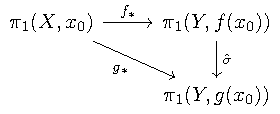
\includegraphics[]{otros/diagrama-prop-6-11.pdf}
    \end{center}
}{
    Sea $[\alpha]\in\pi_1(X,x_0)$, notemos en primer lugar que $f\circ\alpha,g\circ\alpha$ son lazos en torno a los puntos $f(x_0),g(x_0)$ respectivamente. Además sabemos que
    \begin{align*}
        \hat{\sigma} \circ f_{*}([\alpha]) = g_*([\alpha]) \iff  [\overline{\sigma}] * [f \circ \alpha] * [\sigma]  = [g \circ \alpha] \iff \\
        \iff [f \circ \alpha] = [\sigma] * [g \circ \alpha] * [\overline{\sigma}] \iff [f \circ \alpha] = [\sigma * g \circ \alpha * \overline{\sigma}]
    \end{align*}
    por tanto solo hace falta ver que
    \[
    \sigma * g \circ \alpha * \overline{\sigma} \simeq_p f \circ \alpha.
    \]
    Para probar esto último consideremos la homotopía por caminos siguiente
    \[
    G(s,t)=\begin{cases}
        \sigma(3ts) = F(x_0,3ts) & s\in[0,\frac{1}{3}]\\
        F(\alpha(3s-1),t) & s\in[\frac{1}{3},\frac{2}{3}]\\
        \sigma(3t(1-s)) = F(x_0,3t(1-s)) & s\in[\frac{2}{3},1]
    \end{cases}
    \]
    ahora basta notar que $G(s,0)$ es una reparametrización del producto de caminos $\epsilon_{f(x_0)} * (f\circ\alpha) * \epsilon_{f(x_0)}$ mientras que $G(s,1)$ es una reparametrización del producto de caminos $\sigma * (g\circ\alpha) * \overline{\sigma}$, lo que nos permite afirmar que $\epsilon_{f(x_0)} * (f\circ\alpha) * \epsilon_{f(x_0)} \simeq_p \sigma * (g\circ\alpha) * \overline{\sigma}$.

    Finalmente aplicando la \hyperref[prop:propiedades-producto-caminos]{Proposición 3.3.5} obtenemos 
    \[
        f\circ\alpha \simeq_p \epsilon_{f(x_0)} * f\circ\alpha * \epsilon_{f(x_0)} \simeq_p \sigma * g\circ\alpha * \overline{\sigma}
    \]
    como queríamos ver.
}

\corp{
    El grupo fundamental es un invariante homotópico. En efecto, si  
    \[
        f : X \to Y
    \]  
    es una equivalencia de homotopía entre espacios topológicos homotópicamente equivalentes, entonces  
    \[
        f_{*} : \pi_1(X, x_0) \to \pi_1(Y, f(x_0))
    \]  
    es un isomorfismo de grupos.
}{
    Por ser $f$ una equivalencia de homotopía debe existir $g$ tal que
    \[
        g \circ f \simeq Id_X, \quad f \circ g \simeq Id_Y
    \]
    Sea $F_X$ la homotopía entre $Id_X,g \circ f$ y sea $F_Y$ la homotopía entre $Id_Y, f \circ g$. Sea $x_0 \in X$ y sea  $\sigma_X=F_X(x_0,t)$ aplicando la proposición anterior obtenemos:
    \begin{align*}
        \hat{\sigma}_X \circ (Id_X)_* = \hat{\sigma}_X \circ Id_{\pi_1(X,x_0)} = g_* \circ f_*
    \end{align*}
    Como $\hat{\sigma}_X, Id_{\pi_1(X,x_0)}$ son isomorfismos su composición también lo es, por tanto $g_* \circ f_*$ es un isomorfismo, lo que implica que $f_*$ debe ser inyectiva. 
    
    Similarmente, consideremos la aplicación $\sigma_Y=F_Y(f(x_0),t)$, aplicando la proposición anterior obtenemos:
    \begin{align*}
        \hat{\sigma}_Y \circ (Id_Y)_* = \hat{\sigma}_Y \circ Id_{\pi_1(Y,f(x_0))} = f_* \circ g_*
    \end{align*}
    igual que antes $\hat{\sigma}_X \circ Id_{\pi_1(Y,f(x_0))}$ es un isomorfismo, y por tanto $f_*$ debe ser sobreyectiva, lo que finaliza la prueba puesto que ya sabemos que es un homomorfismo. 
}

\corp{
    Si $X$ es un espacio contráctil entonces $X$ es simplemente conexo.
}{
    Si $X$ es contráctil entonces es homotópico a un punto $\{x\}$, como el único lazo en este espacio es el lazo constante, su grupo fundamental es el grupo trivial: $\pi_1(\{x\})\cong(0,+)$. Finalmente, por el corolario anterior el grupo fundamental es un invariante homotópico, y como $X\simeq\{x\}$ hemos de tener
    \[
    \pi_1(X)\cong\pi_1(\{x\})\cong(0,+).
    \]
    Finalmente, el \hyperref[cor:contractil-arcoconexo]{Corolario 3.2.3} nos permite asegurar que $X$ es arcoconexo, lo que prueba que $X$ es simplemente conexo.
}

\clearpage

\section{Aplicaciones recubridoras}

\defn{Aplicación recubridora}{
    Sea $p:E \to B$ una aplicación continua y sobreyectiva. Decimos que $p$ es una aplicación recubridora si para todo $b \in B$ existe un entorno $U\in\E(b)$ tal que
    \[
        p^{-1}(U)=\bigcup_{i \in J} V_i
    \]
    donde los $V_i$ son abiertos disjuntos en $E$ y
    \[
    p|_{V_i}:V_i \to U
    \]
    es un homeomorfismo para todo $i \in J$.
    Se dice que $E$ es un espacio recubridor de $B$. Si $J=\{1,\dots,n\}$ diremos que $p$ es una aplicación recubridora de $n$ hojas.
}

\ex{
    La aplicación $p : \mathbb{R} \to \mathbb{S}^1$ dada por $p(t) = (\cos 2\pi t, \sin 2\pi t)$ es una aplicación recubridora.
}

\pf{
    $p$ es continua por ser composición de funciones continuas, y es sobreyectiva pues todo punto en $\mathbb{S}^1$ puede expresarse en coordenadas polares como $(\cos \theta, \sin \theta)$ para algún $\theta \in \mathbb{R}$, luego $p(\frac{\theta}{2\pi})=b$.

    Sea $b = (\cos \theta, \sin \theta) \in \mathbb{S}^1$. Tomemos el entorno $U = \mathbb{S}^1 \setminus \{-b\}$, entonces
    \[
    p^{-1}(U) = \bigcup_{k \in \mathbb{Z}} \left( k + \frac{\theta}{2\pi} - \frac{1}{2}, k + \frac{\theta}{2\pi} + \frac{1}{2} \right),
    \]
    donde cada $V_k = \left( k + \frac{\theta}{2\pi} - \frac{1}{2}, k + \frac{\theta}{2\pi} + \frac{1}{2} \right)$ es abierto en $\mathbb{R}$ y $p|_{V_k} \colon V_k \to U$ es un homeomorfismo. Los $V_k$ son disjuntos y $p$ restringida a cada $V_k$ es biyectiva, con inversa continua.
}

\ex{
    La aplicación $p : \mathbb{S}^1 \to \mathbb{S}^1$ dada por $p(x, y) = (x^2 - y^2, 2xy)$ (elevar al cuadrado en $\mathbb{C}$) es una aplicación recubridora.
}

\pf{
    $p$ es continua por serlo cada componente, y es sobreyectiva pues dado $b = (\cos \theta, \sin \theta) \in \sphere^1, \theta \in \R$ podemos tomar $(x,y)=(\cos \frac{\theta}{2}, \sin \frac{\theta}{2})$ de manera que
    \[
    p(x,y)=(\cos \frac{\theta}{2} - \sin \frac{\theta}{2}, 2\cos \frac{\theta}{2}\sin \frac{\theta}{2})=(\cos \theta, \sin \theta) = b.
    \]
    
    Además, para cualquier $b \in \mathbb{S}^1$, podemos tomar $U = \mathbb{S}^1 \setminus \{-b\}$. Supongamos ahora que el punto $b$ está en el primer cuadrante, para el resto de cuadrantes podemos razonar de manera similar. Es fácil comprobar que
    \[
    p^{-1}(-b)=\{a,b\},\quad a=(\cos(\theta+\frac{\pi}{2}),\sin(\theta+\frac{\pi}{2})), b=(\cos(\theta+\frac{3\pi}{2}),\sin(\theta+\frac{3\pi}{2}))
    \]
    Entonces es claro que:
    \[
        p^{-1}(U) = V_1 \cup V_2,
    \]
    donde $V_1$ y $V_2$ son los dos hemisferios abiertos de $\mathbb{S}^1$ dados por
    \[
    V_1=\{(\cos\alpha,\sin\alpha) \mid \alpha \in (\theta+\frac{\pi}{2},\theta+\frac{3\pi}{2})\},\quad V_2=\{(\cos\alpha,\sin\alpha) \mid \alpha \in (\theta+\frac{3\pi}{2},2\pi)\cup[0,\theta+\frac{\pi}{2})\}.
    \]
    Cada $V_i$ es un "sector" de $\mathbb{S}^1$ que cubre la mitad del círculo, y $p|_{V_i}$ es un homeomorfismo. Si $b$ no estuviera en el primer cuadrante también obtenemos dos hemisferios abiertos, los detalles se dejan como ejercicio.
}

\propp{}{
    El producto de dos aplicaciones recubridoras es una aplicación recubridora.
}{
    Sean $p_1 \colon E_1 \to B_1$ y $p_2 \colon E_2 \to B_2$ aplicaciones recubridoras. Entonces el producto es
    \[
    p = p_1 \times p_2 \colon E_1 \times E_2 \to B_1 \times B_2, \quad p(e_1, e_2)=(p_1(e_1), p_2(e_2)).
    \]
    Para ver que $p$ es una aplicación recubridora es inmediato que
    $p$ es continua y sobreyectiva porque $p_1$ y $p_2$ lo son.

    Dado $(b_1, b_2) \in B_1 \times B_2$, existen entornos $U_1 \subset B_1$ de $b_1$ y $U_2 \subset B_2$ de $b_2$ tales que:
    \[
    p_1^{-1}(U_1) = \bigcup_{i \in I} V_i^1, \quad p_2^{-1}(U_2) = \bigcup_{j \in J} V_j^2,
    \]
    con los $V_i^1, V_j^2$ disjuntos y tales que $p_1|_{V_i^1} \colon V_i^1 \to U_1$ y $p_2|_{V_j^2} : V_j^2 \to U_2$ son homeomorfismos. Entonces, para $U = U_1 \times U_2$, tenemos:
    \[
    p^{-1}(U) = \bigcup_{(i,j) \in I \times J} V_i^1 \times V_j^2.
    \]
    Cada $V_i^1 \times V_j^2$ es abierto en $E_1 \times E_2$, son disjuntos, y:
    \[
        p|_{V_i^1 \times V_j^2} \colon V_i^1 \times V_j^2 \to U_1 \times U_2
    \]
    es un homeomorfismo porque es producto de homeomorfismos. Por lo tanto, $p_1 \times p_2$ es una aplicación recubridora.
}

\ex{
    Sea $p : \mathbb{R} \to \mathbb{S}^1$ dada por $p(t) = (\cos 2\pi t, \sin 2\pi t)$, entonces $p \times p : \mathbb{R}^2 \to \mathbb{S}^1 \times \mathbb{S}^1$ es una aplicación recubridora sobre el toro.
}

% Faltan las demostraciones de los dos lemas. Están en la clase del 29/04

\lem{Levantamiento de caminos}{
    Sea $p : E \to B$ una aplicación recubridora. Sean $e \in E$, $b \in B$ tales que $p(e) = b$. Para cualquier camino $\alpha : I \to B$ que comienza en $b$, existe un único camino $\tilde{\alpha} : I \to E$ que comienza en $e$ tal que $p \circ \tilde{\alpha} = \alpha$. El camino $\tilde{\alpha}$ se llama levantamiento de $\alpha$.
}

\lem{Levantamiento de homotopías}{
    Sea $p : E \to B$ una aplicación recubridora. Sean $e \in E$, $b \in B$ tales que $p(e) = b$. Para cualquier homotopía por caminos $F : I \times I \to B$ con $F(0,0) = b$, existe una única homotopía por caminos $\tilde{F} : I \times I \to E$ tal que $p \circ \tilde{F} = F$ y $\tilde{F}(0,0) = e$.
}

\propp{}{
    Sea $p : E \to B$ una aplicación recubridora. Sean $e \in E$, $b \in B$ tales que $p(e) = b$. Sean $\alpha$, $\beta$ dos caminos en $B$ comenzando en $b$ y finalizando en un mismo punto $b'$, y sean $\tilde{\alpha}$, $\tilde{\beta}$ sus respectivos levantamientos comenzando en $e$. Si $\alpha \simeq_p \beta$, entonces $\tilde{\alpha} \simeq_p \tilde{\beta}$ y $\tilde{\alpha}$, $\tilde{\beta}$ finalizan en un mismo punto de $E$.
}{
    Supongamos que $\alpha \simeq_p \beta$ y sea $F$ la homotopía por caminos entre $\alpha,\beta$, con $F(0,0)=b$. Por el lema anterior existe una única homotopía por caminos $\tilde{F}$, que cumple $\tilde{F}(0,t)=e,\tilde{F}(1,t)=e'$ para un cierto $e'$. Veamos que es una homotopía entre $\tilde{\alpha},\tilde{\beta}$, en efecto
    \begin{align*}
        p\circ\tilde{F}(s,0)=F(s,0)=\alpha(s)\implies \tilde{F}(s,0)=\tilde{\alpha}(s)\\
        p\circ\tilde{F}(s,1)=F(s,1)=\beta(s)\implies \tilde{F}(s,1)=\tilde{\beta}(s)
    \end{align*}
    y como además mantiene fijos los extremos es una homotopía de caminos, por tanto $\tilde{\alpha}\simeq_p\tilde{\beta}$.
}

\defn{Correspondencia del levantamiento}{
    Sea $p : E \to B$ una aplicación recubridora. Sean $e \in E$, $b \in B$ tales que $p(e) = b$. Definimos la aplicación
    \[
    \Phi : \pi_1(B, b) \to p^{-1}(b)
    \]
    que asigna a cada clase de lazos $[\alpha] \in \pi_1(B, b)$ un elemento de $E$. En concreto, sea $\tilde{\alpha}$ el levantamiento de $\alpha$ que empieza en $e$, entonces ese elemento es
    \[
    \Phi([\alpha]) := \tilde{\alpha}(1).
    \]
}

\propp{}{
    Sea $p : E \to B$ una aplicación recubridora. Sean $e \in E$, $b \in B$ tales que $p(e) = b$.
    \begin{enumerate}
        \item Si $E$ es conexo por caminos, entonces $\Phi$ es sobreyectiva.
        \item Si $E$ es simplemente conexo, entonces $\Phi$ es biyectiva.
    \end{enumerate}
}{
    \begin{enumerate}
        \item Si $E$ es conexo por caminos dado $e' \in p^{-1}(b)$ existe un camino $\tilde{\alpha}$ en $E$ uniendo $e$ con $e'$. Entonces $\alpha=p\circ\tilde{\alpha}$ es un lazo centrado en $b$ con $\Phi([\alpha])=\alpha(1)=e'$ por definición, luego $\Phi$ es sobreyectiva.
        \item Si $E$ es simplemente conexo entonces es conexo por caminos, por lo que el apartado anterior garantiza la sobreyectividad.
        
        Para ver que es inyectiva sean $[\alpha],[\beta]\in\pi_1(B,b)$ tales que $\Phi([\alpha])=\Phi([\beta])$. Sean $\tilde{\alpha},\tilde{\beta}$ los levantamientos empezando en $e$ y terminando en $\tilde{\alpha}(1)=\tilde{\beta}(1)$ dados por la proposición anterior. Como $E$ es simplemente conexo existe una homotopía por caminos $\tilde{F}$ entre $\tilde{\alpha},\tilde{\beta}$, pero entonces $F=p\circ\tilde{F}$ es una homotopía por caminos entre $\alpha,\beta$, por lo que $[\alpha]=[\beta]$.
    \end{enumerate}
}

\thmr{}{grupo-fund-S1}{
    El grupo fundamental de la circunferencia $\mathbb{S}^1$ es isomorfo a $(\mathbb{Z}, +)$.
}

\pf{
    Sea $p:\R \to \sphere^1$ dada por $p(t)=(\cos(2\pi t), \sin(2\pi t))$ y sea $e=0, b=p(0)=(1,0)$. Como ya sabemos, $p$ es una aplicación recubridora. Además, $p^{-1}(b)=\mathbb{Z}$, y como $\R$ es simplemente conexo la aplicación $\Phi$ es una biyección. Veamos que también es un homomorfismo.

    Sean $[\alpha],[\beta]\in\pi_1(\sphere^1,b)$ y sean $\tilde{\alpha},\tilde{\beta}$ los levantamientos empezando en $e$ y terminando en $\tilde{\alpha}(1)=n, \tilde{\beta}(1)=m,\quad n,m\in\mathbb{Z}$. Consideremos el camino en $\R$ dado por
    \[
    \tilde{\tilde{\beta}}:I\to\R, \tilde{\tilde{\beta}}(s)=n+\tilde{\beta}(s)
    \]
    como $p(x+n)=p(x)$ para todo $x\in\R$ entonces $\tilde{\tilde{\beta}}$ es un levantamiento de $\beta$ que comienza en $\tilde{\tilde{\beta}}(0)=n$ en lugar de en $0$. Entonces $\tilde{\alpha}*\tilde{\tilde{\beta}}$ está bien definido ya que
    \[
        \tilde{\alpha}(1)=n=\tilde{\tilde{\beta}}(0)
    \]
    y es un levantamiento de $\alpha*\beta$ que comienza en $0$. Notemos ahora que el punto final de $\tilde{\alpha}*\tilde{\tilde{\beta}}$ es $\tilde{\tilde{\beta}}(1)=n+m$, luego tenemos
    \[
        \Phi([\alpha*\beta])=n+m=\tilde{\alpha}(1)+\tilde{\beta}(1)=\Phi([\alpha])+\Phi([\beta])
    \]
    lo que prueba que $\Phi$ es un homomorfismo.
}

\clearpage
\section{Retractos}

\defn{Retracción, retracto}{
    Sea $A \subset X$ un subconjunto de un espacio topológico $X$. Una retracción de $X$ en $A$ es una aplicación continua $r : X \to A$ tal que $r|_A = Id_A$. Se dice que $A$ es un retracto de $X$.
}

\ex{
    La aplicación $r : \mathbb{R}^{n+1} \setminus \{0\} \to \mathbb{S}^n$ dada por $r(x) = \frac{x}{\|x\|}$ es una retracción, así $\mathbb{S}^n$ es un retracto de $\mathbb{R}^{n+1} \setminus \{0\}$.
}

\lem{}{
    Si $A$ es un retracto de $X$, entonces el homomorfismo inducido $i_* : \pi_1(A, a) \to \pi_1(X, a)$ es inyectivo, para todo $a \in A$, donde $i : A \to X$ es la inclusión.
}

\pf{
    Sea $r$ la retracción de $X$ en $A$. Sean $[\alpha]_A,[\beta]_A\in\pi_1(A, a)$, entonces
    \[
        i_*([\alpha]_A)=i_*([\beta]_A) \implies [i\circ\alpha]_X=[i\circ\beta]_X \implies [\alpha]_X=[\beta]_X.
    \]
    Como $[\alpha]_X=[\beta]_X$ existe una homotopía por caminos $F:I\times I\to X$ entre $\alpha$ y $\beta$. Sea entonces $\tilde{F}:I\times I \to A, \tilde{F} = r \circ F$, que está bien definida porque las imágenes de $\alpha,\beta$ están en $A$. Además $\tilde{F}$ es una homotopía por caminos, luego $[\alpha]_A = [\beta]_A$.
}

\defn{Retracto de deformación}{
    Sea $A \subset X$ un retracto de $X$. Decimos que $A$ es un retracto de deformación de $X$ si la aplicación identidad $Id_X$ es homotópica a $i \circ r$, con $r$ una retracción de $X$ en $A$, de forma que cada punto de $A$ permanece fijo por la homotopía. En particular, $A \simeq X$.
}

\ex{
    $\mathbb{S}^n$ es un retracto de deformación de $\mathbb{R}^{n+1} \setminus \{0\}$.
}

% Falta ver que $r(x) = \frac{x}{\|x\|}$ es homotópica a lo otro 

\corp{
    Sea $A$ un retracto de deformación de $X$. Para todo $a \in A$, el homomorfismo inducido $i_* : \pi_1(A, a) \to \pi_1(X, a)$ por la inclusión es un isomorfismo.
}{
    Como $A$ es un retracto de deformación de $X$ sabemos que $i \circ r \simeq Id_X$, y además es inmediato que $r \circ i = Id_A$. Veamos que $i_*$ es sobreyectiva y habremos terminado, puesto que ya sabemos que es un homomorfismo y que es inyectiva.

    Sea $[\alpha]_X \in \pi_1(X, a)$ y sea
    \[
        \tilde{\alpha}:I\to A,\quad \tilde{\alpha}(s)=r(\alpha(s))
    \]
    entonces
    \[
        i_*([\tilde{\alpha}]_A)=[i\circ\tilde{\alpha}]_X=[(i\circ r)\circ \alpha]_X=[\alpha]_X
    \]
    donde la última igualdad se da porque $i \circ r \simeq Id_X$, luego $i \circ r \circ \alpha \simeq Id_X \circ \alpha \simeq \alpha$.
}

\corp{
    $\pi_1(\mathbb{R}^{n+1} \setminus \{0\}) \cong \pi_1(\mathbb{S}^n)$, para todo $n \geq 1$.
}{
    Por el ejemplo anterior $\sphere^n$ es un retracto de deformación de $\mathbb{R}^{n+1} \setminus \{0\}$, luego $i_*$ es el isomorfismo buscado entre $\pi_1(\mathbb{R}^{n+1} \setminus \{0\})$ y $\pi_1(\mathbb{S}^n)$.
}

\clearpage

\section{Teorema de Seifert-van Kampen}

\thm{Teorema de Seifert-van Kampen (versión reducida)}{
    Supongamos que $X = U \cup V$, donde $U$ y $V$ son abiertos y $U \cap V \neq \emptyset$ es conexo por caminos. Sean $i : U \to X$ y $j : V \to X$ las inclusiones. Para cada $x_0 \in U \cap V$, las imágenes de los homomorfismos inducidos $i_*$ y $j_*$ generan el grupo $\pi_1(X, x_0)$.
}

\pf{
    Queremos ver que dado $[\alpha]\in\pi_1(X, x_0)$ se tiene que 
    \[
        [\alpha]=[\beta_1 * \dots * \beta_n]
    \]
    con cada $\beta_k$ contenido en $U$ o en $V$.

    Existe una subdivisión de $[0,1]$ de la forma $0=a_0<a_1<\dots<a_n=1$ tal que $\alpha(a_i)\in U \cap V$ y $\alpha([a_{i-1},a_{i}])$ está contenido en $U$ o en $V$.

    Definamos $\alpha_i$ como un camino que cubre el trozo de $\alpha$ en el intervalo $[a_{i-1},a_{i}]$ haciendo
    \[
    \alpha_i(t)=\alpha(a_{i-1}+t(a_{i}-a_{i-1})).
    \]
    Es inmediato entonces que 
    \[
    \alpha \simeq_p \alpha_1 * \dots * \alpha_n.
    \]
    Cada curva $\alpha_i$ es un camino uniendo puntos de $U\cap V$, que es conexo por caminos. Por tanto, existe $\gamma_i$ un camino contenido en $U\cap V$ uniendo $x_0$ con $\alpha(a_i)$ . Como $\alpha(a_0)=x_0=\alpha(a_n)$, los arcos $\gamma_1,\gamma_n$ son constantes.

    Finalmente, definamos los arcos $\beta_i=\gamma_{i-1} * \alpha_i * \overline{\gamma_i}$, entonces se tiene que $\beta_i$ es un lazo en $x_0$ y además
    \[
        \beta_1 * \beta_2 * \dots * \beta_n \simeq_p \alpha_1 * \dots * \alpha_n \simeq_p \alpha
    \]
    lo que nos permite concluir 
    \[
        [\alpha]=[\beta_1 * \dots * \beta_n]
    \]
    como queríamos ver.
}

\rmkb{
    Es fácil visualizar el teorema en el caso de los lazos simples. Si tomamos un punto $x_0 \in U\cap V$ y un lazo simple $\alpha$ centrado en $x_0$, entonces siempre podemos dividir este camino en dos lazos distintos $\alpha_1,\alpha_2$ de manera que $\alpha_1$ está en $U$ y $\alpha_2$ está en $V$, y además $[\alpha]=[\alpha_1 * \alpha_2].$
}

\corp{%
    Sea $X = U \cup V$ con $U,\,V\subseteq X$ abiertos tales que $U$ y $V$ son conexos por caminos y simplemente conexos, y $U\cap V \neq \emptyset$ con $U\cap V$ conexo por caminos. Entonces $X$ es simplemente conexo.
}{
    Sea $x_{0}\in U\cap V$.  Como $U$ y $V$ son conexos por caminos y $U \cap V \neq \emptyset$ entonces $X = U\cup V$ es conexo por caminos, lo que nos permite identificar $\pi_{1}(X)\cong\pi_{1}(X,x_{0})$.

    Por el teorema de Seifert-van Kampen las inclusiones $i:U\hookrightarrow X$ y $j:V\hookrightarrow X$ inducen homomorfismos $i_{*}$ y $j_{*}$ cuyas imágenes generan $\pi_{1}(X,x_{0})$.

    Como $U$ y $V$ son simplemente conexos, $\pi_{1}(U,x_{0})=\pi_{1}(V,x_{0})=\{1\}$, de modo que $\operatorname{Im}i_{*}=\operatorname{Im}j_{*}=\{1\}$.

    Finalmente el subgrupo generado por el elemento triviales es el grupo trivial, luego
    \[
        \pi_{1}(X,x_{0})=\langle\{1\}\rangle=\{1\}.
    \]
    Por tanto $X$ es simplemente conexo.
}

\corp{
    La esfera $\mathbb{S}^n$ es simplemente conexa para $n \geq 2$.
}{
    Sean $p=(0,\dots,1)\in\R^{n+1}$ y $q=(0,\dots,-1)\in\R^{n+1}$, entonces $\sphere^n\setminus\{p\}$ es homeomorfa a $\R^n$, por tanto simplemente conexa. De igual manera, $\sphere^n\setminus\{q\}$ es homeomorfa a $\R^n$ y por tanto simplemente conexa. Finalmente notemos que
    \[
    \left( \sphere^n\setminus\{p\} \right) \cap \left( \sphere^n\setminus\{q\} \right) \neq \emptyset, \left( \sphere^n\setminus\{p\} \right) \cup \left( \sphere^n\setminus\{q\}\right) = \sphere^n
    \]
    por tanto, por el corolario anterior, $\sphere^n$ es simplemente conexa.
}

\thm{}{
    Sean $X$ e $Y$ dos espacios topológicos y fijemos puntos $x_0 \in X$, $y_0 \in Y$. Entonces
    \[
    \pi_1(X \times Y, (x_0, y_0)) \cong \pi_1(X, x_0) \times \pi_1(Y, y_0).
    \]
}
\pf{
    Queremos construir un isomorfismo de grupos
    \[
        \Phi : \pi_1(X \times Y, (x_0, y_0)) \longrightarrow \pi_1(X, x_0) \times \pi_1(Y, y_0).
    \]
    Consideremos las proyecciones canónicas $p : X \times Y \to X$ y $q : X \times Y \to Y$. Estas aplicaciones son continuas y, por lo tanto, inducen homomorfismos entre los grupos fundamentales:
    \begin{align*}
        p_* &: \pi_1(X \times Y, (x_0, y_0)) \longrightarrow \pi_1(X, x_0) \\
        q_* &: \pi_1(X \times Y, (x_0, y_0)) \longrightarrow \pi_1(Y, y_0).
    \end{align*}
    Definimos la aplicación $\Phi$ de la siguiente manera: para cualquier lazo $[\alpha] \in \pi_1(X \times Y, (x_0, y_0))$,
    \[
        \Phi([\alpha]) := (p_*([\alpha]), q_*([\alpha])) = ([p \circ \alpha]_X, [q \circ \alpha]_Y).
    \]
    Para demostrar que $\Phi$ es un isomorfismo, verificaremos que es un homomorfismo y que es biyectiva.

    \paragraph{1. $\Phi$ es un homomorfismo}
    Sean $[\alpha], [\beta] \in \pi_1(X \times Y, (x_0, y_0))$. Entonces,
    \begin{align*}
        \Phi([\alpha] * [\beta]) &= \Phi([\alpha * \beta]) \\
        &= (p_*([\alpha * \beta]), q_*([\alpha * \beta])) \\
        &= ([p \circ (\alpha * \beta)]_X, [q \circ (\alpha * \beta)]_Y).
    \end{align*}
    Dado que $[p \circ (\alpha * \beta)]_X = [p \circ \alpha]_X * [p \circ \beta]_X$ y análogamente $[q \circ (\alpha * \beta)]_Y = [q \circ \alpha]_Y * [q \circ \beta]_Y$, se sigue que
    \begin{align*}
        p_*([\alpha * \beta]) &= [p \circ \alpha * p \circ \beta]_X = [p \circ \alpha]_X * [p \circ \beta]_X = p_*([\alpha]) * p_*([\beta]) \\
        q_*([\alpha * \beta]) &= [q \circ \alpha * q \circ \beta]_Y = [q \circ \alpha]_Y * [q \circ \beta]_Y = q_*([\alpha]) * q_*([\beta]).
    \end{align*}
    Por lo tanto,
    \begin{align*}
        \Phi([\alpha] * [\beta]) &= (p_*([\alpha]) * p_*([\beta]), q_*([\alpha]) * q_*([\beta])) \\
        &= (p_*([\alpha]), q_*([\alpha])) * (p_*([\beta]), q_*([\beta])) \\
        &= \Phi([\alpha]) * \Phi([\beta]).
    \end{align*}
    Así, $\Phi$ es un homomorfismo de grupos.

    \paragraph{2. $\Phi$ es inyectiva}
    Sabemos que un homomorfismo es inyectivo si y solo si su núcleo es trivial. En este caso, el núcleo de $\Phi$ está dado por
    \[
        Ker(\Phi) = \{[\alpha] \in \pi_1(X \times Y, (x_0, y_0)) : [p \circ \alpha] = [\varepsilon_{x_0}], [q \circ \alpha] = [\varepsilon_{y_0}]\}.  
    \]

    Supongamos que $\alpha$ es un lazo en $(x_0, y_0)$ con $[\alpha] \in Ker(\Phi)$. Esto implica que $p \circ \alpha \simeq_p \varepsilon_{x_0}$ y $q \circ \alpha \simeq_q \varepsilon_{y_0}$. Sean $H$ y $G$ las respectivas homotopías. Entonces, definimos

    \[
        F((x, y), t) = (H(x, t), G(y, t)),
    \]
    que es homotopía entre $\alpha$ y el lazo constante en $(x_0, y_0)$. Por lo tanto, $[\alpha] = [\varepsilon_{(x_0, y_0)}]$, lo que implica que el núcleo de $\Phi$ es trivial.
    \paragraph{3. $\Phi$ es sobreyectiva}
    Sea $\gamma_1$ lazo en $X$ centrado en $x_0$ y $\gamma_2$ lazo en $Y$ centrado en $y_0$. Buscamos $[\alpha] \in \pi_1(X \times Y, (x_0, y_0))$ tal que $\Phi([\alpha]) = ([\gamma_1], [\gamma_2])$. 

    Basta tomar $\alpha(s) = (\gamma_1(s), \gamma_2(s))$ para $s \in [0, 1]$ y observar que cumple las condiciones. 

    \vspace{0.5cm}
    Hemos visto que $\Phi$ es un homomorfismo de grupos, inyectivo y sobreyectivo, por lo que es un isomorfismo. 
}   

\corp{
    $\pi_1(\mathbb{S}^1 \times \mathbb{S}^1) \cong \mathbb{Z} \times \mathbb{Z}$.
}{
    El resultado es inmediato si notamos que $\sphere^1$ es conexo por caminos, luego $\sphere^1\times\sphere^1$ también, y por tanto los grupos fundamentales no dependen del punto escogido. Además, por el \hyperref[thm:grupo-fund-S1]{Teorema 3.6.8}
    \[
    \pi_1(\mathbb{S}^1) \cong \mathbb{Z} 
    \]
    por lo que aplicando el teorema anterior se obtiene el resultado.
}

\propp{}{
    El grupo fundamental del plano proyectivo $\mathbb{RP}^2$ es $\mathbb{Z}_2$.
}{
    Consideremos $\mathbb{RP}^2$ como el espacio cociente en $\sphere^2$ al identificar puntos opuestos. En tal caso la aplicación
    \[
        p: \sphere^2 \to \mathbb{RP}^2,\quad p(x)=[x]
    \]
    es una aplicación recubridora de dos hojas (la demostración de que lo es queda como ejercicio). Como $\sphere^2$ es simplemente conexa la correspondencia del levantamiento
    \[
        \Phi: \pi_1(\mathbb{RP}^2,x)\to p^{-1}([x])
    \]
    es una biyección. Ahora notemos que $\mathbb{RP}^2$ es conexo por caminos, luego el grupo fundamental no depende del punto escogido, y además $p^{-1}([x])=\{x,-x\}$, por lo que $\pi_1(\mathbb{RP}^2)$ tiene solo dos elementos. Finalmente, un resultado bien conocido sobre teoría de grupos nos permite afirmar que todos los grupos de dos elementos son isomorfos a $\mathbb{Z}_2$, luego
    \[
        \pi_1(\mathbb{RP}^2)\cong\mathbb{Z}_2
    \]
    como queríamos ver.
}

\propp{}{
    El grupo fundamental de la figura ocho $\mathbb{S}^1 \lor \mathbb{S}^1$ es no abeliano (grupo libre de dos generadores).
}{
    Pendiente.
}

\corp{
    El grupo fundamental del plano doblemente agujereado es no abeliano.
}{
    Pendiente.
}

\corp{
    El grupo fundamental del doble toro $\mathbb{T}^2 \#\mathbb{T}^2$ es no abeliano.
}{
    Pendiente.
}